\documentclass[hidelinks,12pt]{article}
\usepackage[left=0.25cm,top=1cm,right=0.25cm,bottom=1cm]{geometry}
%\usepackage[landscape]{geometry}
\textwidth = 20cm
\hoffset = -1cm
\usepackage[utf8]{inputenc}
\usepackage[spanish,es-tabla, es-lcroman]{babel}
\usepackage[autostyle,spanish=mexican]{csquotes}
\usepackage[tbtags]{amsmath}
\usepackage{nccmath}
\usepackage{amsthm}
\usepackage{amssymb}
\usepackage{mathrsfs}
\usepackage{graphicx}
\usepackage{subfig}
\usepackage{caption}
%\usepackage{subcaption}
\usepackage{standalone}
\usepackage[outdir=./Imagenes/]{epstopdf}
\usepackage{siunitx}
\usepackage{physics}
\usepackage{color}
\usepackage{float}
\usepackage{hyperref}
\usepackage{multicol}
\usepackage{multirow}
%\usepackage{milista}
\usepackage{anyfontsize}
\usepackage{anysize}
%\usepackage{enumerate}
\usepackage[shortlabels]{enumitem}
\usepackage{capt-of}
\usepackage{bm}
\usepackage{mdframed}
\usepackage{relsize}
\usepackage{placeins}
\usepackage{empheq}
\usepackage{cancel}
\usepackage{pdfpages}
\usepackage{wrapfig}
\usepackage[flushleft]{threeparttable}
\usepackage{makecell}
\usepackage{fancyhdr}
\usepackage{tikz}
\usepackage{bigints}
\usepackage{menukeys}
\usepackage{tcolorbox}
\tcbuselibrary{breakable}
\usepackage{scalerel}
\usepackage{pgfplots}
\usepackage{pdflscape}
\pgfplotsset{compat=1.16}
\spanishdecimal{.}
\renewcommand{\baselinestretch}{1.5} 
\renewcommand\labelenumii{\theenumi.{\arabic{enumii}})}

\newcommand{\python}{\texttt{python}}
\newcommand{\textoazul}[1]{\textcolor{blue}{#1}}
\newcommand{\azulfuerte}[1]{\textcolor{blue}{\textbf{#1}}}
\newcommand{\funcionazul}[1]{\textcolor{blue}{\textbf{\texttt{#1}}}}

\newcommand{\pderivada}[1]{\ensuremath{{#1}^{\prime}}}
\newcommand{\sderivada}[1]{\ensuremath{{#1}^{\prime \prime}}}
\newcommand{\tderivada}[1]{\ensuremath{{#1}^{\prime \prime \prime}}}
\newcommand{\nderivada}[2]{\ensuremath{{#1}^{(#2)}}}


\newtheorem{defi}{{\it Definición}}[section]
\newtheorem{teo}{{\it Teorema}}[section]
\newtheorem{ejemplo}{{\it Ejemplo}}[section]
\newtheorem{propiedad}{{\it Propiedad}}[section]
\newtheorem{lema}{{\it Lema}}[section]
\newtheorem{cor}{Corolario}
\newtheorem{ejer}{Ejercicio}[section]

\newlist{milista}{enumerate}{2}
\setlist[milista,1]{label=\arabic*)}
\setlist[milista,2]{label=\arabic{milistai}.\arabic*)}
\newlength{\depthofsumsign}
\setlength{\depthofsumsign}{\depthof{$\sum$}}
\newcommand{\nsum}[1][1.4]{% only for \displaystyle
    \mathop{%
        \raisebox
            {-#1\depthofsumsign+1\depthofsumsign}
            {\scalebox
                {#1}
                {$\displaystyle\sum$}%
            }
    }
}
\def\scaleint#1{\vcenter{\hbox{\scaleto[3ex]{\displaystyle\int}{#1}}}}
\def\scaleoint#1{\vcenter{\hbox{\scaleto[3ex]{\displaystyle\oint}{#1}}}}
\def\scaleiiint#1{\vcenter{\hbox{\scaleto[3ex]{\displaystyle\iiint}{#1}}}}
\def\bs{\mkern-12mu}

\newcommand{\Cancel}[2][black]{{\color{#1}\cancel{\color{black}#2}}}


\usepackage{courier}
\usepackage{listingsutf8}
\usepackage{listings}
\usepackage{xcolor}
\usepackage{textcomp}
\usepackage{color}
\definecolor{deepblue}{rgb}{0,0,0.5}
\definecolor{brown}{rgb}{0.59, 0.29, 0.0}
\definecolor{OliveGreen}{rgb}{0,0.25,0}
% \usepackage{minted}

\DeclareCaptionFont{white}{\color{white}}
\DeclareCaptionFormat{listing}{\colorbox{gray}{\parbox{0.98\textwidth}{#1#2#3}}}
\captionsetup[lstlisting]{format=listing,labelfont=white,textfont=white}
\renewcommand{\lstlistingname}{Código}


\definecolor{Code}{rgb}{0,0,0}
\definecolor{Keywords}{rgb}{255,0,0}
\definecolor{Strings}{rgb}{255,0,255}
\definecolor{Comments}{rgb}{0,0,255}
\definecolor{Numbers}{rgb}{255,128,0}

\makeatletter

\newif\iffirstchar\firstchartrue
\newif\ifstartedbyadigit
\newif\ifprecededbyequalsign

\newcommand\processletter
{%
  \ifnum\lst@mode=\lst@Pmode%
    \iffirstchar%
        \global\startedbyadigitfalse%
      \fi
      \global\firstcharfalse%
    \fi
}

\newcommand\processdigit
{%
  \ifnum\lst@mode=\lst@Pmode%
      \iffirstchar%
        \global\startedbyadigittrue%
      \fi
      \global\firstcharfalse%
  \fi
}

\lst@AddToHook{OutputOther}%
{%
  \lst@IfLastOtherOneOf{=}
    {\global\precededbyequalsigntrue}
    {}%
}

\lst@AddToHook{Output}%
{%
  \ifprecededbyequalsign%
      \ifstartedbyadigit%
        \def\lst@thestyle{\color{orange}}%
      \fi
    \fi
  \global\firstchartrue%
  \global\startedbyadigitfalse%
  \global\precededbyequalsignfalse%
}

\lstset{ 
language=Python,                % choose the language of the code
basicstyle=\footnotesize\ttfamily,       % the size of the fonts that are used for the code
numbers=left,                   % where to put the line-numbers
numberstyle=\scriptsize,      % the size of the fonts that are used for the line-numbers
stepnumber=1,                   % the step between two line-numbers. If it is 1 each line will be numbered
numbersep=5pt,                  % how far the line-numbers are from the code
backgroundcolor=\color{white},  % choose the background color. You must add \usepackage{color}
showspaces=false,               % show spaces adding particular underscores
showstringspaces=false,         % underline spaces within strings
showtabs=false,                 % show tabs within strings adding particular underscores
frame=single,   		% adds a frame around the code
tabsize=2,  		% sets default tabsize to 2 spaces
captionpos=t,   		% sets the caption-position to bottom
breaklines=true,    	% sets automatic line breaking
breakatwhitespace=false,    % sets if automatic breaks should only happen at whitespace
escapeinside={| |},  % if you want to add a comment within your code
stringstyle =\color{OliveGreen},
otherkeywords={as, np.array, np.concatenate, np.linspace, linspace, interpolate.interp1d, kind, plt.plot, .copy, np.arange, np.cos, np.pi, lw, ls, label, splrep, splev, plt.legend, loc, plt.title, plt.ylim, plt.show, sign, math.ceil, math.log, np.sqrt, np.exp, np.zeros, plt.xlabel, plt.ylabel, plt.xlim, np.identity, random, np.dot, np.outer, np.diagonal },             % Add keywords here
keywordstyle = \color{blue},
commentstyle = \color{darkcerulean},
identifierstyle = \color{black},
literate=%
         {á}{{\'a}}1
         {é}{{\'e}}1
         {í}{{\'i}}1
         {ó}{{\'o}}1
         {ú}{{\'u}}1
%
%keywordstyle=\ttb\color{deepblue}
%fancyvrb = true,
}

\lstdefinestyle{FormattedNumber}{%
    literate={0}{{\textcolor{red}{0}}}{1}%
             {1}{{\textcolor{red}{1}}}{1}%
             {2}{{\textcolor{red}{2}}}{1}%
             {3}{{\textcolor{red}{3}}}{1}%
             {4}{{\textcolor{red}{4}}}{1}%
             {5}{{\textcolor{red}{5}}}{1}%
             {6}{{\textcolor{red}{6}}}{1}%
             {7}{{\textcolor{red}{7}}}{1}%
             {8}{{\textcolor{red}{8}}}{1}%
             {9}{{\textcolor{red}{9}}}{1}%
             {.0}{{\textcolor{red}{.0}}}{2}% Following is to ensure that only periods
             {.1}{{\textcolor{red}{.1}}}{2}% followed by a digit are changed.
             {.2}{{\textcolor{red}{.2}}}{2}%
             {.3}{{\textcolor{red}{.3}}}{2}%
             {.4}{{\textcolor{red}{.4}}}{2}%
             {.5}{{\textcolor{red}{.5}}}{2}%
             {.6}{{\textcolor{red}{.6}}}{2}%
             {.7}{{\textcolor{red}{.7}}}{2}%
             {.8}{{\textcolor{red}{.8}}}{2}%
             {.9}{{\textcolor{red}{.9}}}{2}%
             {\ }{{ }}{1}% handle the space
         ,%
          %mathescape=true
          escapeinside={__}
          }




%Este paquete permite manejar los encabezados del documento
\usepackage{fancyhdr}
%hay que definir el ambiente de la página
\pagestyle{fancy}
\fancyhf{}
%\fancyheadoffset{0.05\textwidth}
%aqui va el texto para todas las paginas l--> izquierda, r--> derecha, hay un C--> para centrar el texto deseado
%\lhead{Curso de Física Computacional}
\fancyhead[L]{\nouppercase{\leftmark}}
\fancyhead[R]{\nouppercase{\rightmark}}
\fancyfoot[C]{\thepage}

%define el ancho de la linea que separa el encabezado del cuerpo del texto
\renewcommand{\headrulewidth}{0.5pt}
\setlength{\parskip}{1em}
\renewcommand{\baselinestretch}{1.5}
\interfootnotelinepenalty=8000
\usepackage{hyperref}
%esta parte define el color del marco que aparece en las hiperreferencias.
\definecolor{links}{HTML}{2A1B81}
\hypersetup{colorlinks,linkcolor=,urlcolor=links}

\spanishdecimal{.}
%\marginsize{1.5cm}{1.5cm}{1.5cm}{1.5cm}


\author{M. en C. Gustavo Contreras Mayén.}
\title{Manejo de archivos de datos con \python \\ \begin{Large} Curso de Física Computacional\end{Large} \\
\begin{small}
\texttt{curso.fisica.comp@gmail.com}
\end{small}}
\date{ }

\begin{document}

\maketitle
\fontsize{14}{14}\selectfont

\section{Los archivos de datos con \python.}
\subsection{Consideraciones.}

Una tarea muy común y frecuente en el ámbito de la Física Computacional, será el manejo de archivos de datos para su proceso y análisis.
\par
Como una primera tarea que hay que atender en el desarrollo de prácticas de programación bajo cualquier lenguaje, es la generación de un archivo de datos con una serie de características necesarias:
\begin{enumerate}
\item Una estructura de construcción, que permita la posterior lectura del archivo.
\item La codificación de los caracteres que conforman los datos, este punto es crítico si además de números, se incluyen o manejan cadenas de texto (el manejo de acentos y ciertos caracteres es crítico si no se considera este elemento)
\end{enumerate}
\subsection{Estructura del archivo.}
Debemos de elegir anticipadamente el tipo de archivo que vamos a generar, ya que de esta forma, al momento de definir el código, se implementará la estructura del archivo.
\par
Quien reciba el archivo para su procesamiento, análisis, etc. debe de conocer el tipo de estructura que lleva. En el posible caso de que no avisemos esta información, el usuario del archivo, deberá de hacer una revisión preliminar del archivo para identificar la estrucutura. En el caso de que nosotros seamos los usuarios de un archivo de datos y no tengamos la informción, será nuestra tarea entonces, hacer la revisión de la estructura interna del archivo.
\par
Existen diversos formatos para los archivos de texto, a continuación se describen cuatro de los más conocidos:
\begin{table}[H]
\centering
\begin{tabular}{| m{3.5cm} | m{10cm} |}
\hline
\textbf{Tipo de archivo} & \multicolumn{1}{>{\centering\arraybackslash} m{10cm}|}{\textbf{Descripción}} \\ \hline
txt & Texto plano que representa sólo caracteres (o cadenas), excluye cualquier tipo de metadatos. \\ \hline
csv & Valores separados por coma (Comma-separated values), utiliza comas (u otro delimitador) para estructurar los datos almacenados, permitiendo guardarlos en un formato tipo tabla. \\ \hline
HMTL & Lenguaje de marcado de hipertexto (HyperText Markup Language) almacena los datos de manera estrucutrada, se utiliza comúnmente en páginas web. \\ \hline
JSON  & Notación de objeto de JavaScript (JavaScript Object Notation) es un formato sencillo y eficiente, siendo un formato para almacenar y transferir datos. \\ \hline
\end{tabular}
\end{table}
Al momento en que compartan el archivo, se recomienda elaborar un archivo \textbf{README}, que contiene información acerca de otros archivos ya sea en un directorio o un archivo comprimido.
\par
Es una forma de documentación de software, consiste en un archivo de texto plano llamado \textbf{READ.ME}, \textbf{README.TXT}, \textbf{README.md} (para un archivo markdown), \textbf{README.1ST} o simplemente \textbf{README}.
\par
El nombre del archivo es generalmente escrito en mayúsculas. En los sistemas Unix-like, generalmente los nombres se escriben en minúscula, y esto hace que en un listado de archivos salga primero el archivo \textbf{README}.
\section{Creando un archivo de datos.}
Con \python\ será una tarea muy frecuente el generar un archivo de datos y compartirlo con otros usuarios.
\par
Las instrucciones para crear el archivo son sencillas de implemantar en el código, toma en cuenta lo siguiente:
\begin{enumerate}
\item El archivo de datos se va a crear en la misma carpeta en donde se está ejecutando el archivo de \python, es decir, el archivo con extensión \texttt{*.py}
\item Un archivo de datos requiere de la \enquote{apertura} de un espacio en memoria, para que con una instrucción, se \enquote{escriban} los datos en el archivo.
\item Una vez que se completa la tarea de escribir los datos, hay que cerrar el espacio de memoria.
\end{enumerate}
\subsection{El código con \python.}
Del ejercicio que se realizó para resolver el cálculo de valores a través de la interpolación de Newton:
\begin{lstlisting}[style= FormattedNumber, basicstyle=\linespread{1.1}\ttfamily=\normal, columns=fullflexible]
from newtonPoli import coeficientes, evaluaPoli
import numpy as np

resultados = open('DatosNewton.dat','w')

xDatos = np.array([0.15,2.30,3.15,4.85,6.25,7.95])
yDatos = np.array([4.79867,4.49013,4.2243,3.47313,2.66674,1.51909])

a = coeficientes(xDatos, yDatos)

print ('{:^3} \t {:^7} \t {:^7} \t {:<11}'.format('x', 'yInterpol', 'yExacta', 'Err relativo'))
print ('-'*55)


for x in np.arange(0.0, 8.1, 0.5):
    y = evaluaPoli(a, xDatos, x)
    yExacta = 4.8 * np.cos(np.pi*x/20.0)
    print ('{:1.1f} \t {:1.5f} \t {:1.5f} \t {:1.5E}'.format(x, y, yExacta, abs(yExacta - y)/yExacta*100))
    resultados.write ('{:1.1f} \t {:1.5f} \t {:1.5f} \n'.format(x, y, yExacta))
    
resultados.close()
\end{lstlisting}
En la línea 4 del código, se indica la función \azulfuerte{open}, que se requiere para \enquote{abrir} el espacio para el archivo, recibe como primer argumento el nombre del archivo y su extensión: \emph{DatosNewton.dat}, nótese que la extensión que hemos dejado, es \emph{*.dat}, se puede utilizar libremente el tipo de extensión \emph{*.txt}, \emph{*.inf}, \emph{*.text}, \emph{*.data}, etc.
\par
Lo relevante de la extensión es que el sistema operativo con el que trabajen, pueda distinguir que se trata de un archivo de datos en texto plano.
\par
Como segundo argumento, se indica la \textit{'w'} en la misma línea 4 del código, indica que se va a realizar la instrucción \textit{write}, lo que permitirá escribir en el archivo. Como punto importante hay que señalar, que en caso de que el archivo \textit{DatosNewton.dat} no exista, \python\ creará un archivo nuevo, en caso de que ya exista, lo va a sobre-escribir.
\par
En la línea 19 del código, se señala la instrucción que va a escribir los datos en el archivo: \texttt{resultados.write(argumento)}, en donde en el caso del ejercicio, el argumento consiste en una cadena de formato para tres columnas, cada una de ellas, separada mediante una tabulación (\texttt{\textbackslash t}) y al final de la cadena de formato, se incluye un salto de línea (\textbackslash n), que permitirá que en el siguiente ciclo del bucle, se escriba en otra línea del archivo, los valores que se calculan en esa iteración.
\par
Una vez concluido el proceso de iteración, o el proceso donde se calcularon los valores del problema, se debe de cerrar el espacio del archivo, o de lo contrario tendremos un error. Para cerrar el objeto tipo \emph{file}, se ocupa la función \azulfuerte{nombreobjeto.close()}, como lo vemos en la línea de código 21.
\par
Con estas instrucciones de manejo de un archivo, ya contamos en nuestro directorio de un archivo de datos que podremos utilizar posteriormente. Toma en cuenta que no se han incluido cabeceras de las columnas, en el ejercicio, las líneas 11 y 12, muestran en la terminal una cabecera con el nombre de la columna y una línea que separa a modo de tabla.
\par
La pregunta natural es: ¿podremos incluir cabeceras o información adicional en nuestro archivo y que no interfiera con la recuperación de los datos?
\section{Recuperando los datos.}
Siguiendo con el ejercicio de la interpolación de Newton y contando ya con un archivo de datos: \emph{DatosNewton.dat}, ahora nos aplicaremos para recuperar los datos y con ellos, generar una gráfica con la librería \azulfuerte{\texttt{matplotlib}}.
\subsection{Extraer los datos del archivo.}
Revisemos el código que se requiere para primero obtener los datos del archivo y posteriomente usar la rutina ya conocida para graficar.
\begin{lstlisting}[style= FormattedNumber, basicstyle=\linespread{1.1}\ttfamily=\normal, columns=fullflexible]
import matplotlib.pyplot as plt
import csv

x = []
yi = []
ye = []


with open('DatosNewton.dat', 'r') as csvfile:
    plots = csv.reader(csvfile, delimiter = '\t')
    for row in plots:
       x.append(float(row[0]))
       yi.append(float(row[1]))
       ye.append(float(row[2]))
       

plt.plot(x, yi, label='Polinomio Newton', ls = 'dashed')
plt.plot(x, ye, label='Valor exacto', color = 'red')
plt.title('Grafica de los datos de un archivo')
plt.legend(loc = 1)
plt.show()
\end{lstlisting}
En la línea 2 se importa la librería \emph{csv} que permitirá el manejo de un archivo de este tipo; como se mencionó en el apartado anterior, se requiere conocer el tipo de delimitador que se utilizó para generar el archivo.
\par
Se requieren tres listas en donde vamos a almacenar los valores del archivo:
\begin{enumerate}
\item Un arreglo para representar la variable independiente, en este caso $x$.
\item Un arreglo para los valores de interpolación $yi$.
\item Un arreglo para los valores evaluados con la función exacta $ye$.
\end{enumerate}
En la línea 9 del código mediante la instrucción \azulfuerte{\texttt{with open}}, se declara un objeto de tipo \texttt{file}, al que se le da un alias: \texttt{csvfile}. Necesita al menos de dos argumentos: el nombre del archivo y el tipo de operación que se va a ejecutar, en nuestro ejemplo, vamos a usar \texttt{r}, que corresponde a la acción de leer los datos del archivo. Toma en cuenta que con la misma función \azulfuerte{\texttt{open}}	se pueden realizar las tareas de escribir un archivo y de leer los datos contenidos en el mismo.
\par
Una vez definido el objeto \texttt{file}, se necesita recuperar los elementos contenidos, para ello usamos la función \azulfuerte{\texttt{csv.reader}}, con dos argumentos: el nombre del objeto file y el delimitador con el que se guardó el archivo. El delimitador es un argumento necesario, como se mencionó previamente para los archivos de datos, puede usar un delimitador:
\begin{itemize}
\item Espacio en blanco.
\item Tabulación.
\item Coma.
\item Guión.
\end{itemize}
De acuerdo al delimitador utilizado, se debe de indicar en el respectivo argumento, para nuestro ejemplo \texttt{delimiter = $'\backslash t'$}.
\subsection{Almacenando temporalmente los datos.}
Posteriormente tenemos un ciclo \azulfuerte{\texttt{for}}, mediante el cual se van agregando los elementos del archivo en cada lista, toma en cuenta que los datos que están en el archivo, a pesar de que la representación que vemos de ellos, correspondan a números, \python\ los guardó como \textbf{\texttt{strings}}, siendo necesario la conversión a un tipo de dato \textbf{float} para su uso en la gráfica.
\par
A partir de la línea 17 del código, se presenta la rutina de graficación ya conocida y manejada en el curso de Física Computacional.
\par
El resultado obtenido es la siguiente gráfica:
\begin{figure}[H]
\centering
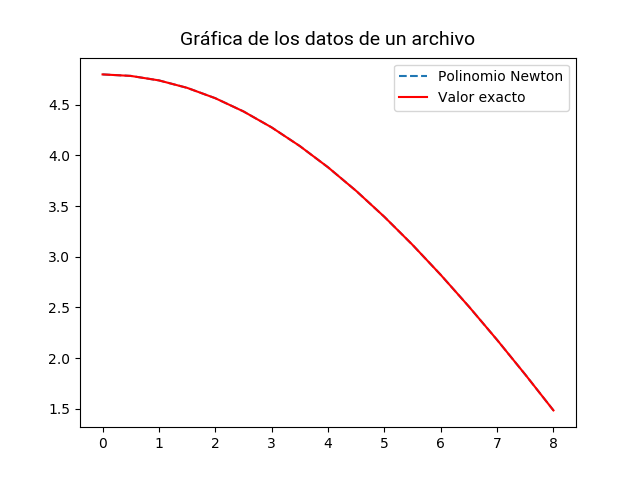
\includegraphics[scale=0.9]{Imagenes/Archivos_01}
\caption{Gráfica generada a partir de los datos en un archivo.}
\end{figure}
Las opciones que hemos visto para el manejo de archivos son las básicas, podrás extender su uso e implementación cuando revises la respectiva documentación.
\par
El potencial que se tiene con \python\ para el manejo de arhivos es muy grande, ya que se pueden manejar archivos de datos y analizarlos sin necesidad de cambiar de formatos, por ejemplo, un archivo de datos en Excel (que en algunos casos suele ser un tipo de archivo aceptado para el ámbito científico) se puede operar con librerías especializadas como \texttt{\textbf{pandas}} que contiene funciones que operan directamente en los archivos.
\end{document} 